\chapter{Chapter Four}
\section{Discussion}
The number of cases with biased versus unbiased $Z_{DR}$ at CWKR was evenly split, with five each.
\subsection{Diagnosing $Z_{DR}$ Bias}
\subsubsection{$Z_{DR}$ Statistics}
The unbiased cases are given in Table \ref{unbiased}.
\begin{table}[h]
    \caption{Statistics of cases with unbiased $Z_{DR}$, using the KDE > 2 constrained $Z_{DR}$ dataset.}\label{unbiased}
    \begin{center}
    \begin{tabular}{|l|c|c|c|c|c|c|c|}
    \hline
     &
    \multicolumn{4}{|c|}{CWKR $Z_{DR}$ (dB)} &
    \multicolumn{3}{|c|}{KBUF $Z_{DR}$ (dB)} \\
    \hline
     Event & Bias & Min & Max & Range & Bias & Min & Max & Range\\
    \hline\hline
    2014-01-18 & -0.10 & 0.19 & 0.5 & 0.31 & -0.40 & 0.21 & 0.65 & 0.44 \\
    \hline
    2014-01-23 & -0.06 & 0.00 & 0.19 & 0.19 & -0.40 & -0.04 & 0.34 & 0.38\\
    \hline
    2015-01-06 &  0.00  & 0.44  & 0.62  & 0.18 & 0.41 & 0.66 & 0.25 \\
    \hline
    2015-01-07 & -0.04  & 0.13  & 0.44  & 0.32 & -0.01 & 0.61 & 0.62 \\ 
    \hline
    2016-02-10 & -0.06  & -0.06  & 0.06  & 0.12 &-0.02 & 0.10 & 0.12  \\ 
    \hline\hline
    Mean & -- & 0.14 & 0.36 & 0.22 & 0.11 & 0.47 & 0.362 \\
    \hline
    \end{tabular}
    \end{center}
\end{table}
The biased cases are given in Table \ref{biased}.
\begin{table}[h]
    \caption{Statistics of cases with biased $Z_{DR}$, using the KDE $ \geq 2$ constrained $Z_{DR}$ dataset.}\label{biased}
    \begin{center}
    \begin{tabular}{|l|c|c|c|c|c|c|c|}
    \hline
     &
    \multicolumn{4}{|c|}{CWKR $Z_{DR}$ (dB)} &
    \multicolumn{4}{|c|}{KBUF $Z_{DR}$ (dB)} \\
    \hline
     Event & Bias & Min & Max & Range & Bias & Min & Max & Range\\
    \hline\hline
    2014-02-01 & 0.22 & 0.25 & 0.69 & 0.44 & -0.20 &-0.05 & 0.51 & 0.56 \\
    \hline
    2015-02-06 & 0.28 & 0.25 & 0.56 & 0.31 & -0.10 & -0.12 & 0.37 & 0.49\\
    \hline
    2015-02-14 & 0.38 & 0.31  & 0.75  & 0.44 & -0.10 & -0.09 & 0.41 & 0.50 \\
    \hline
    2015-02-18 & 0.30 & 0.44  & 0.81  & 0.37 & -0.10 & -0.09 & 0.66 & 0.75 \\ 
    \hline
    2016-12-15 & -0.47 & -0.25  & 0.12  & 0.37 & -0.40 & -0.25 & 0.45 & 0.70  \\ 
    \hline\hline
    Mean & -- & 0.20 & 0.59 & 0.39 & -- & -0.12 & 0.48 & 0.60 \\
    \hline
    \end{tabular}
    \end{center}
\end{table}
\begin{figure}[H]
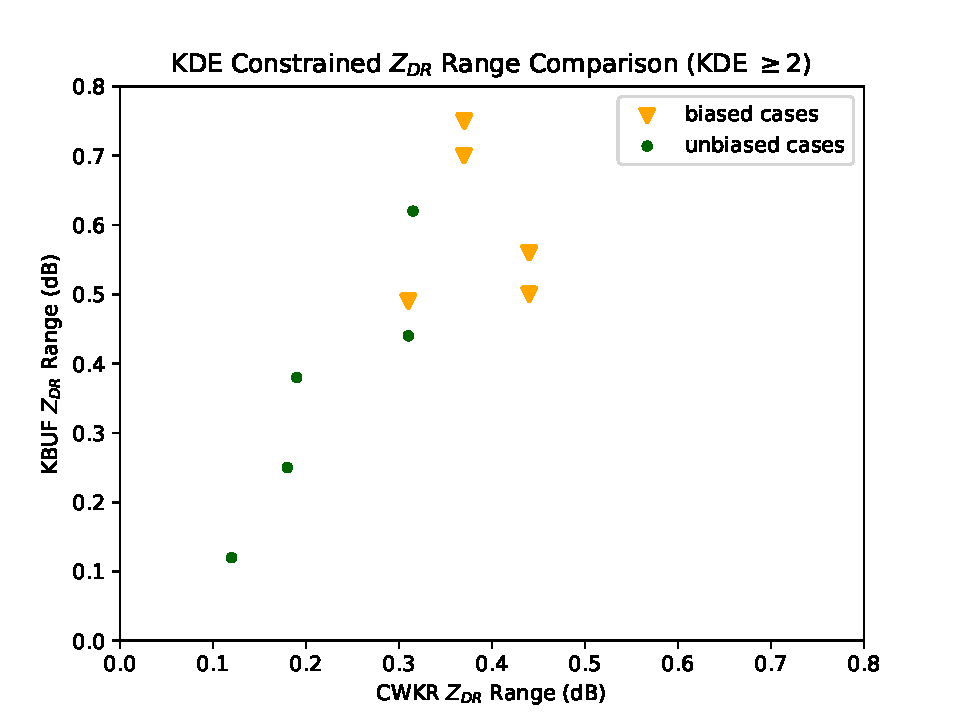
\includegraphics[width=\textwidth]{bias_range}
\caption{Blah} 
\label{fig:bias_compare}
\end{figure}
\subsubsection{Beam Volume Differences}
The source of the bias could be due to large differences in beam volumes between radars, in combination with a large gradients of $Z_{DR}$ with height. \citep{Ryzhkov2007} found a similiar result to this, in that cross-beam gradients of $Z_{DR}$ can produce significant biases. 
\begin{figure}[H]
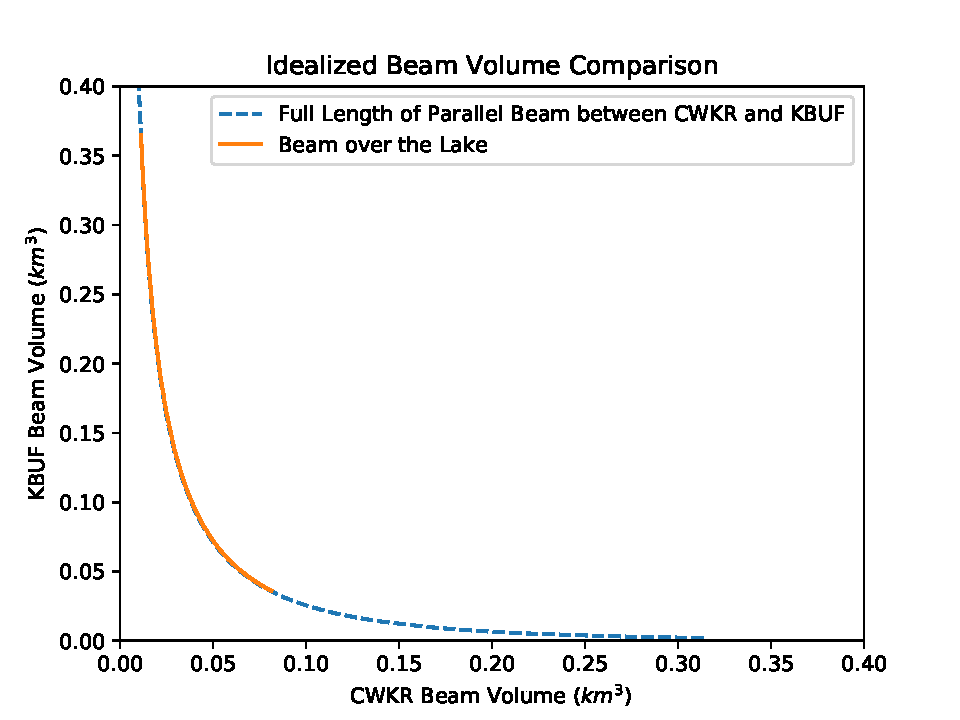
\includegraphics[width=\textwidth]{ideal_beam}
\caption{Blah} 
\label{fig:bias_compare}
\end{figure}